% Trying to break the document up a bit.  This command simply inserts the contents of the file at this point.  It contains the document license, preamble, and title page: things that aren't likely to change more than once.  This can be used to separate discrete parts of a document into files that are easier to edit at one time.
%%%%%%%%%%%%%%%%%%%%%%%%%%%%%%%%%%%%%%%%%%%%%%%%%%%%%%%%%%%%%%%%%%%%%%
% This layout was adapted from one found at latextemplates.com which
% was adapted from another.
%
% License: CC BY-NC-SA 3.0
% (http://creativecommons.org/licenses/by-nc-sa/3.0/)
%
% Original header:
%
% This is a LaTeX version of the sample laboratory report from
% Virginia Tech's copyrighted 08-09 CHEM 1045/1046 lab manual.
% Reproduction of this one appendix section for academic purposes
% should fall under fair use.
%
%%%%%%%%%%%%%%%%%%%%%%%%%%%%%%%%%%%%%%%%%%%%%%%%%%%%%%%%%%%%%%%%%%%%%%

\documentclass{article}

\usepackage{graphicx}
% \usepackage[acronym]{glossaries} % Lets us use acronyms
\usepackage{multicol}
\usepackage{amsmath}
\usepackage{siunitx} % SI units in math mode
\usepackage{subcaption}

\author{}
\title{ELEC-313 \\ Lab 5: CMOS Circuits\\ }
\date{\today}

% \loadglsentries{acronyms} % Actually loads 'acronyms.tex'
% \makeglossaries

\begin{document}

\maketitle

\begin{center}
  \begin{tabular}{lr}
    Date Performed: & October 16, 2013 \\
    Partners:       & Charles Pittman    \\
    & Stephen Wilson     \\
  \end{tabular}
\end{center}

\newpage

\tableofcontents
\listoffigures
\listoftables
\newpage

% Number the enumerate environment (unordered lists) by letter:
\renewcommand{\labelenumi}{\alph{enumi}.}

\section{Objective}

The objective is to plot the output characteristic of a common-emitter transistor circuit, and use it to determine the current gain and output conductance.

\section{Equipment}

\begin{tabular}{ll}
  \centering
  Transistor: 2N7000               & Power supply: HP E3631A            \\
  Function generator: HP 33120 & Multimeter: HP 34401A              \\
  Oscilloscope: Agilent 54622D & Capacitors: \SI{0.1}{\micro\farad} \\
  \multicolumn{2}{l}{Resistors: \SI{100}{\ohm}, \SI{300}{\ohm}, \SI{470}{\ohm}, \SI{1}{\kilo\ohm} (x2) \SI{33}{\kilo\ohm}, \SI{100}{\kilo\ohm} (x2)} \\
\end{tabular}

\section{Schematics}

\begin{figure}[hbtp]
  \centering
  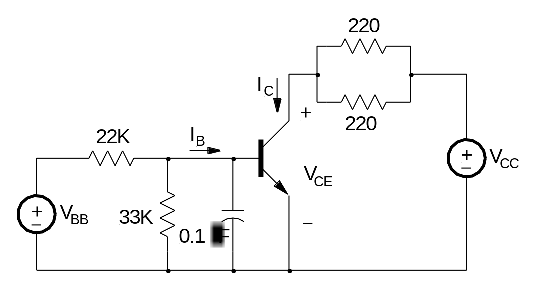
\includegraphics[width=0.6\textwidth]{circuit}
  \caption{\label{fig:circuit} Common-emitter transistor circuit}
\end{figure}

% \begin{figure}[hbtp]
%   \centering
%   \begin{subfigure}[b]{0.5\textwidth}
%     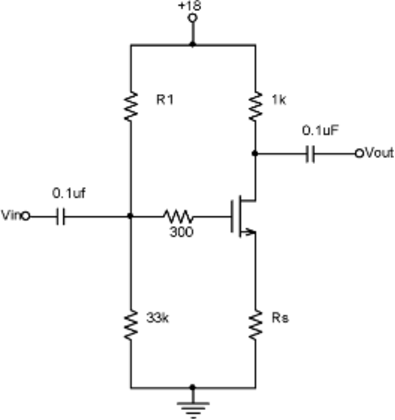
\includegraphics[width=\textwidth]{common-source}
%     \caption{\label{schem:common-source} Common-source amplifier}
%   \end{subfigure}%
%   ~
%   \begin{subfigure}[b]{0.5\textwidth}
%     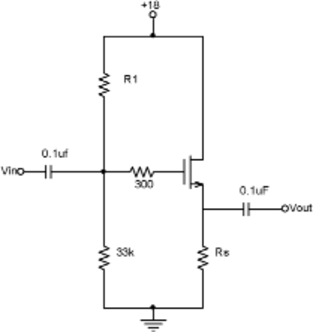
\includegraphics[width=\textwidth]{source-follower}
%     \caption{\label{schem:source-follower} Source-follower amplifier}
%   \end{subfigure}
%   \caption{\label{fig:schematics} Circuits used in this lab. $R_1=\SI{100}{\kilo\ohm}$,  $R_s=\SI{470}{\ohm}$}
% \end{figure}

\section{Procedure}

The following steps were observed to plot the output characteristic of a common emitter transistor circuit:

\begin{enumerate}
\item Construct the circuit of Figure~\ref{fig:circuit}.  Use the +\SI{6}{V} power supply for $V_{BB}$ and the +\SI{25}{V} supply for $V_{CC}$.  Be sure to keep the connection distance between the capacitor and the transistor short.  Use the HP multimeter to measure the base current ($I_B$) on the source side of the capacitor and Fluke multimeters to measure the collector voltage and current ($V_{CE}$ and $I_C$).
\item Adjust $V_{BB}$ so that base current ($I_B$) is \SI{20}{\micro\ampere}.
\item Adjust $V_{CC}$ from 0.5 -- \SI{1.5}{V} in \SI{0.25}{V} steps, then from 2 -- \SI{20}{V} in \SI{2}{V} steps.
\item At each step measure the collector current, $I_C$, and the collector-to-emitter voltage, $V_{CE}$.  If $I_B$ has drifted, readjust $V_{BB}$ before recording the values of $I_C$ and $V_{CE}$.
\item Adjust $V_{BB}$ for a base current of \SI{50}{\micro\ampere}, \SI{80}{\micro\ampere}, and \SI{100}{\micro\ampere}.  Repeat steps 3 and 4 at each $I_B$ value.
\end{enumerate}

\section{Results}

\begin{table}[hbtp]
  \centering
  \begin{tabular}{cccc}
    $V_{CC}$ & $I_C$     & $V_{CE}$ & $\beta$ \\
    (\si{V}) & (\si{mA}) & (\si{V}) &         \\
    \hline
    0.50     & 0.232     & 0.454    & 11.60   \\
    0.75     & 0.233     & 0.705    & 11.65   \\
    1.00     & 0.234     & 0.954    & 11.70   \\
    1.25     & 0.237     & 1.204    & 11.85   \\
    1.50     & 0.237     & 1.454    & 11.85   \\
    2        & 0.242     & 1.954    & 12.10   \\
    4        & 0.25      & 3.95     & 12.30   \\
    6        & 0.25      & 5.95     & 12.60   \\
    8        & 0.26      & 7.95     & 12.75   \\
    10       & 0.26      & 9.96     & 12.85   \\
    12       & 0.26      & 11.95    & 13.10   \\
    14       & 0.27      & 13.94    & 13.30   \\
    16       & 0.27      & 15.95    & 13.40   \\
    18       & 0.27      & 17.95    & 13.50   \\
    20       & 0.27      & 19.95    & 13.70   \\
  \end{tabular}
  \caption{\label{tab:1} $I_B = $ \SI{20}{\micro\ampere}}
\end{table}

\begin{table}[hbtp]
  \centering
  \begin{tabular}{cccc}
    $V_{CC}$ & $I_C$     & $V_{CE}$ & $\beta$ \\
    (\si{V}) & (\si{mA}) & (\si{V}) &         \\
    \hline
    0.50     & 2.73      & 0.178    & 54.60   \\
    0.75     & 4.34      & 0.236    & 86.80   \\
    1.00     & 4.96      & 0.41     & 99.20   \\
    1.25     & 4.95      & 0.662    & 99.00   \\
    1.50     & 4.97      & 0.91     & 99.40   \\
    2        & 4.98      & 1.41     & 99.60   \\
    4        & 5.15      & 3.39     & 103.00  \\
    6        & 5.25      & 5.38     & 105.00  \\
    8        & 5.39      & 7.36     & 107.80  \\
    10       & 5.58      & 9.34     & 111.60  \\
    12       & 5.77      & 11.31    & 115.40  \\
    14       & 5.97      & 13.28    & 119.40  \\
    16       & 6.21      & 15.26    & 124.20  \\
    18       & 6.45      & 17.23    & 129.00  \\
    20       & 6.69      & 19.20    & 133.80  \\
  \end{tabular}
  \caption{\label{tab:2}$I_B = $ \SI{50}{\micro\ampere}}
\end{table}

\begin{table}[hbtp]
  \centering
  \begin{tabular}{cccc}
    $V_{CC}$ & $I_C$     & $V_{CE}$ & $\beta$ \\
    (\si{V}) & (\si{mA}) & (\si{V}) &         \\
    \hline
    0.50     & 3.08      & 0.135    & 38.50   \\
    0.75     & 4.95      & 0.163    & 61.88   \\
    1.00     & 6.8       & 0.191    & 85.00   \\
    1.25     & 8.58      & 0.229    & 107.25  \\
    1.50     & 9.1       & 0.421    & 113.75  \\
    2        & 9.4       & 0.881    & 117.50  \\
    4        & 10.79     & 2.71     & 134.88  \\
    6        & 11.03     & 4.68     & 137.88  \\
    8        & 11.45     & 6.63     & 143.13  \\
    10       & 11.99     & 8.56     & 149.88  \\
    12       & 12.72     & 10.47    & 159.00  \\
    14       & 13.41     & 12.39    & 167.63  \\
    16       & 14.20     & 14.29    & 177.50  \\
    18       & 15.05     & 16.20    & 188.13  \\
    20       & 15.85     & 18.10    & 198.13  \\
  \end{tabular}
  \caption{\label{tab:3}$I_B = $ \SI{80}{\micro\ampere}}
\end{table}

\begin{table}[hbtp]
  \centering
  \begin{tabular}{cccc}
    $V_{CC}$ & $I_C$     & $V_{CE}$ & $\beta$ \\
    (\si{V}) & (\si{mA}) & (\si{V}) &         \\
    \hline
    0.50     & 3.21      & 0.12     & 32.10   \\
    0.75     & 5.11      & 0.143    & 51.10   \\
    1.00     & 7.02      & 0.164    & 70.20   \\
    1.25     & 8.93      & 0.186    & 89.30   \\
    1.5      & 10.79     & 0.214    & 107.90  \\
    2        & 10.33     & 0.77     & 103.30  \\
    4        & 11.33     & 2.67     & 113.30  \\
    6        & 13.95     & 4.34     & 139.50  \\
    8        & 15.63     & 6.14     & 156.30  \\
    10       & 16.60     & 8.02     & 166.00  \\
    12       & 17.98     & 9.95     & 179.80  \\
    14       & 19.20     & 11.70    & 192.00  \\
    16       & 20.70     & 13.69    & 207.00  \\
    18       & 22.40     & 15.53    & 224.00  \\
    20       & 23.80     & 17.37    & 238.00  \\
    \end{tabular}
    \caption{\label{tab:4}$I_B = $ \SI{100}{\micro\ampere}}
\end{table}

\begin{table}[hbtp]
  \centering
  \begin{tabular}{cc}
    $I_B$ (\si{\micro\ampere}) & $\beta_{avg}$ \\
    \hline
    20                         & 12.55         \\
    50                         & 105.85        \\
    80                         & 132.00        \\
    100                        & 137.99        \\
  \end{tabular}
  \caption{\label{tab:beta_IB} Average values of $\beta$ per $I_B$}
\end{table}

\begin{figure}[hbtp]
  \centering
  \resizebox{1.0\textwidth}{!}{% GNUPLOT: LaTeX picture with Postscript
\begingroup
  \makeatletter
  \providecommand\color[2][]{%
    \GenericError{(gnuplot) \space\space\space\@spaces}{%
      Package color not loaded in conjunction with
      terminal option `colourtext'%
    }{See the gnuplot documentation for explanation.%
    }{Either use 'blacktext' in gnuplot or load the package
      color.sty in LaTeX.}%
    \renewcommand\color[2][]{}%
  }%
  \providecommand\includegraphics[2][]{%
    \GenericError{(gnuplot) \space\space\space\@spaces}{%
      Package graphicx or graphics not loaded%
    }{See the gnuplot documentation for explanation.%
    }{The gnuplot epslatex terminal needs graphicx.sty or graphics.sty.}%
    \renewcommand\includegraphics[2][]{}%
  }%
  \providecommand\rotatebox[2]{#2}%
  \@ifundefined{ifGPcolor}{%
    \newif\ifGPcolor
    \GPcolortrue
  }{}%
  \@ifundefined{ifGPblacktext}{%
    \newif\ifGPblacktext
    \GPblacktextfalse
  }{}%
  % define a \g@addto@macro without @ in the name:
  \let\gplgaddtomacro\g@addto@macro
  % define empty templates for all commands taking text:
  \gdef\gplbacktext{}%
  \gdef\gplfronttext{}%
  \makeatother
  \ifGPblacktext
    % no textcolor at all
    \def\colorrgb#1{}%
    \def\colorgray#1{}%
  \else
    % gray or color?
    \ifGPcolor
      \def\colorrgb#1{\color[rgb]{#1}}%
      \def\colorgray#1{\color[gray]{#1}}%
      \expandafter\def\csname LTw\endcsname{\color{white}}%
      \expandafter\def\csname LTb\endcsname{\color{black}}%
      \expandafter\def\csname LTa\endcsname{\color{black}}%
      \expandafter\def\csname LT0\endcsname{\color[rgb]{1,0,0}}%
      \expandafter\def\csname LT1\endcsname{\color[rgb]{0,1,0}}%
      \expandafter\def\csname LT2\endcsname{\color[rgb]{0,0,1}}%
      \expandafter\def\csname LT3\endcsname{\color[rgb]{1,0,1}}%
      \expandafter\def\csname LT4\endcsname{\color[rgb]{0,1,1}}%
      \expandafter\def\csname LT5\endcsname{\color[rgb]{1,1,0}}%
      \expandafter\def\csname LT6\endcsname{\color[rgb]{0,0,0}}%
      \expandafter\def\csname LT7\endcsname{\color[rgb]{1,0.3,0}}%
      \expandafter\def\csname LT8\endcsname{\color[rgb]{0.5,0.5,0.5}}%
    \else
      % gray
      \def\colorrgb#1{\color{black}}%
      \def\colorgray#1{\color[gray]{#1}}%
      \expandafter\def\csname LTw\endcsname{\color{white}}%
      \expandafter\def\csname LTb\endcsname{\color{black}}%
      \expandafter\def\csname LTa\endcsname{\color{black}}%
      \expandafter\def\csname LT0\endcsname{\color{black}}%
      \expandafter\def\csname LT1\endcsname{\color{black}}%
      \expandafter\def\csname LT2\endcsname{\color{black}}%
      \expandafter\def\csname LT3\endcsname{\color{black}}%
      \expandafter\def\csname LT4\endcsname{\color{black}}%
      \expandafter\def\csname LT5\endcsname{\color{black}}%
      \expandafter\def\csname LT6\endcsname{\color{black}}%
      \expandafter\def\csname LT7\endcsname{\color{black}}%
      \expandafter\def\csname LT8\endcsname{\color{black}}%
    \fi
  \fi
  \setlength{\unitlength}{0.0500bp}%
  \begin{picture}(7200.00,5040.00)%
    \gplgaddtomacro\gplbacktext{%
      \csname LTb\endcsname%
      \put(726,440){\makebox(0,0)[r]{\strut{}0mA}}%
      \csname LTb\endcsname%
      \put(726,1307){\makebox(0,0)[r]{\strut{}5mA}}%
      \csname LTb\endcsname%
      \put(726,2174){\makebox(0,0)[r]{\strut{}10mA}}%
      \csname LTb\endcsname%
      \put(726,3041){\makebox(0,0)[r]{\strut{}15mA}}%
      \csname LTb\endcsname%
      \put(726,3908){\makebox(0,0)[r]{\strut{}20mA}}%
      \csname LTb\endcsname%
      \put(726,4775){\makebox(0,0)[r]{\strut{}25mA}}%
      \csname LTb\endcsname%
      \put(858,220){\makebox(0,0){\strut{}0 V}}%
      \csname LTb\endcsname%
      \put(1453,220){\makebox(0,0){\strut{}2 V}}%
      \csname LTb\endcsname%
      \put(2047,220){\makebox(0,0){\strut{}4 V}}%
      \csname LTb\endcsname%
      \put(2642,220){\makebox(0,0){\strut{}6 V}}%
      \csname LTb\endcsname%
      \put(3236,220){\makebox(0,0){\strut{}8 V}}%
      \csname LTb\endcsname%
      \put(3831,220){\makebox(0,0){\strut{}10 V}}%
      \csname LTb\endcsname%
      \put(4425,220){\makebox(0,0){\strut{}12 V}}%
      \csname LTb\endcsname%
      \put(5020,220){\makebox(0,0){\strut{}14 V}}%
      \csname LTb\endcsname%
      \put(5614,220){\makebox(0,0){\strut{}16 V}}%
      \csname LTb\endcsname%
      \put(6209,220){\makebox(0,0){\strut{}18 V}}%
      \csname LTb\endcsname%
      \put(6803,220){\makebox(0,0){\strut{}20 V}}%
    }%
    \gplgaddtomacro\gplfronttext{%
      \csname LTb\endcsname%
      \put(5816,4602){\makebox(0,0)[r]{\strut{}$I_B = $SI{20}{microampere}}}%
      \csname LTb\endcsname%
      \put(5816,4382){\makebox(0,0)[r]{\strut{}$I_B = $SI{50}{microampere}}}%
      \csname LTb\endcsname%
      \put(5816,4162){\makebox(0,0)[r]{\strut{}$I_B = $SI{80}{microampere}}}%
      \csname LTb\endcsname%
      \put(5816,3942){\makebox(0,0)[r]{\strut{}$I_B = $SI{100}{microampere}}}%
    }%
    \gplbacktext
    \put(0,0){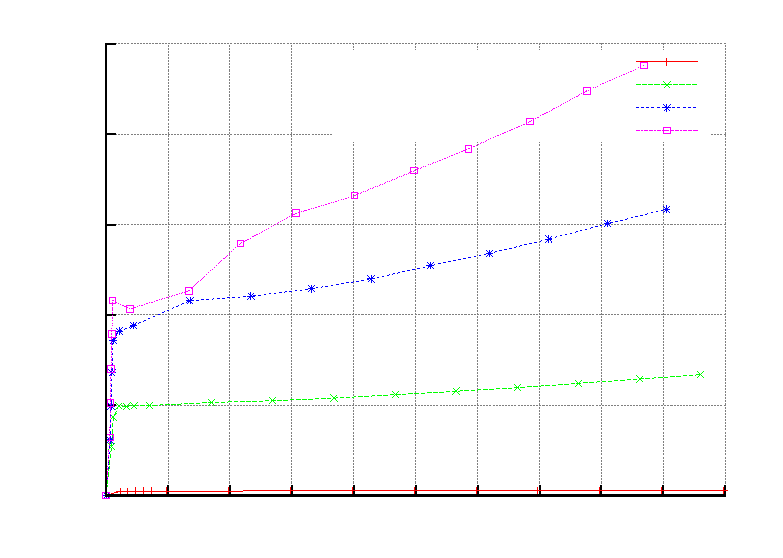
\includegraphics{graph}}%
    \gplfronttext
  \end{picture}%
\endgroup
}
  \caption{\label{fig:graph} $V_{CE}$ vs. $I_C$}
\end{figure}

\begin{table}[hbtp]
  \centering
  \begin{tabular}{ccc}
    $I_B$                & $I_C$     & $\beta$ \\
    (\si{\micro\ampere}) & (\si{mA}) &         \\
    \hline
    20                   & 0.25      & 12.26   \\
    50                   & 5.20      & 104.00  \\
    80                   & 11.10     & 138.75  \\
    100                  & 14.67     & 146.68  \\
  \end{tabular}
  \caption{\label{tab:da2a1}$V_{CE} = $ \SI{5}{V}}
\end{table}

\begin{table}[hbtp]
  \centering
  \begin{tabular}{ccc}
    $I_B$                & $I_C$     & $\beta$ \\
    (\si{\micro\ampere}) & (\si{mA}) &         \\
    \hline
    20                   & 0.26      & 12.97   \\
    50                   & 5.64      & 112.84  \\
    80                   & 12.47     & 155.88  \\
    100                  & 18.00     & 180.00  \\
  \end{tabular}
  \caption{\label{tab:da2a2}$V_{CE} = $ \SI{10}{V}}
\end{table}

\begin{table}[hbtp]
  \centering
  \begin{tabular}{ccc}
    $I_B$                & $I_C$     & $\beta$ \\
    (\si{\micro\ampere}) & (\si{mA}) &         \\
    \hline
    20                   & 0.27      & 13.32   \\
    50                   & 6.18      & 123.61  \\
    80                   & 14.50     & 181.25  \\
    100                  & 22.93     & 229.30  \\
  \end{tabular}
  \caption{\label{tab:da2a3}$V_{CE} = $ \SI{15}{V}}
\end{table}

\begin{table}[hbtp]
  \centering
  \begin{tabular}{cc}
    $V_{CE}$ (\si{V}) & $\beta_{avg}$ \\
    \hline
    5                 & 100.42        \\
    10                & 115.42        \\
    15                & 136.87        \\
  \end{tabular}
  \caption{\label{tab:beta_VCE} Average values of $\beta$ per $V_{CE}$}
\end{table}

\begin{table}[hbtp]
  \centering
  \begin{tabular}{ccc}
    $I_B$                & $h_{oe}$ & $r_o$            \\
    (\si{\micro\ampere}) &          & (\si{\kilo\ohm}) \\
    \hline
     20                  & 1.700E-6 & 58.82            \\
     50                  & 9.950E-5 & 10.10            \\
     80                  & 3.669E-4 & 2.726            \\
    100                  & 7.412E-4 & 1.349            \\
  \end{tabular}
  \caption{\label{tab:hoe} $h_{oe}$ vs. $r_o$}
\end{table}

\newpage
\section{Conclusion}
\label{sec:conclusion}

As shown in Figure~\ref{fig:graph}, the family of curves associated with the four $I_B$ currents loosely follow the typical plots of Bipolar Junction Transistors (BJTs).  The mode of operation of the transistor transitions to the “forward-active mode” when $V_{CE}$ is  greater than approximately \SI{0.2}{V}.  Also, as $I_B$ increases, the slope of the $I_C$ to $V_{CE}$ increases.

Tables \ref{tab:1}, \ref{tab:2}, \ref{tab:3}, and \ref{tab:4} show that as $I_B$ increases, the ratio of $I_C$ to $I_B$ (current gain, $\beta$) also increases.  This change in $\beta$ seems to ``taper off'' as $I_B$ increases such that if one were to plot mean $\beta$ vs. $I_B$, it would resemble logarithmic growth.  If one were to plot mean $\beta$ vs. $V_{CE}$ , I suspect it would resemble exponential growth though there is minimal evidence to prove this, considering only three data points are provided in Tables \ref{tab:da2a1}, \ref{tab:da2a2}, and \ref{tab:da2a3}.

Figure ?? shows the slope of each of the family of curves for $V_{CE}$ values greater than \SI{3}{V}.  The output conductance ($h_{oe}$) was conducted with the slope of each of the four the trend line equations and Equation~\ref{eq:hoe}.  As $I_B$ increased, $h_{oe}$ increased.   %Therefore, as $I_B$ increased, current gain $\beta$ because the output resistance $r_o$ decreased.

\section{Equations}

% LaTeX sees blank lines as a start of another paragraph.  To avoid
% unnecessary vertical spaces between equations, and still visually
% separate in source, put a comment between them.
%
\begin{equation}
  \label{eq:beta}
  \beta = \frac{I_C}{I_B}
\end{equation}
%
\begin{equation}
  \label{eq:hoe}
  h_{oe} \approx \frac{1}{r_o} = \frac{\Delta I_C}{\Delta V_{CE}}
\end{equation}
%
% \begin{equation}
%   \label{eqn:percent_diff}
%   \%_{diff} = \frac{|measured - theoretical|}{theoretical} \times 100\%
% \end{equation}

\end{document}
